\documentclass[12pt,a4paper]{article}
\usepackage[UTF8]{ctex}     %先引入ctex
\usepackage[utf8]{inputenc} %再引入inputenc
\usepackage{graphicx}
\usepackage{lazylatex}
\usepackage{amsmath}
\usepackage{bookmark}
\usepackage{enumerate}
\usepackage{array}
\usepackage{xfp}
\usepackage{colortbl}
\usepackage{tikz}

\tcbuselibrary{documentation}
\graphicspath{{img/}}
% 边距
\geometry{left=2.0cm,right=2.0cm,top=2.0cm,bottom=3.0cm}
% 大题
\newenvironment{problems}{\begin{list}{}{\renewcommand{\makelabel}[1]{\textbf{##1}\hfil}}}{\end{list}}
% 小题
\newenvironment{steps}{\begin{list}{}{\renewcommand{\makelabel}[1]{##1.\hfil}}}{\end{list}}
% 答
\providecommand{\ans}{\textbf{答}:~}
% 解
\providecommand{\sol}{\textbf{解}.~}

\newcommand{\allpart}{20}
\providecommand{\blk}[2]{\framebox[\fpeval{round(#2/\allpart*\textwidth*0.8,2)}pt]{$P_#1$}}

\begin{document}
\title{\normalsize \underline{操作系统(D)}\\\LARGE第 8 次作业}
\author{李子龙 518070910095}
\date{\today}
\maketitle

\begin{problems}
    \item[8.3] Consider the following snapshot of a system:
     
    \begin{tabular}{cccc}
         & \underline{\emph{Allocation}} & \underline{\emph{Max}} &  \underline{\emph{Available}}\\
         & $ABCD$ & $ABCD$ & $ABCD$\\
    $T_0$ & 0012 & 0012& 1520\\
    $T_1$ & 1000 & 1750& \\
    $T_2$ & 1354 & 2356& \\
    $T_3$ & 0632 & 0652& \\
    $T_4$ & 0014 & 0656&
    \end{tabular} 

    Answer the following questions using the banker's algorithm:
    \begin{steps}
        \item[a] What is the content of the matrix \emph{Need}?
         
        \sol \begin{tabular}{cc}
            & \underline{\emph{Need}} \\
            & $ABCD$ \\
        $T_0$ & 0000 \\
        $T_1$ & 0750 \\
        $T_2$ & 1002 \\
        $T_3$ & 0020 \\
        $T_4$ & 0642
        \end{tabular} 
        \item[b] Is the system in a safe state?
        
        \sol \begin{tabular}{cc}
          Sequence  & \underline{\emph{Available}} \\
            & $A,B,C,D$ \\
        $T_0$ & 1,5,3,2 \\
        $T_2$ & 2,8,8,6 \\
        $T_1$ & 3,8,8,6 \\
        $T_3$ & 3,14,11,8\\
        $T_4$ & 3,14,12,12
        \end{tabular} 

        找到安全序列 $\langle T_0,T_2,T_1,T_3,T_4\rangle $,所以系统处于安全状态。
        \item[c] If a request from thread $T_1$ arrives for (0,4,2,0), can the request be granted immediately?
        
        \sol 如果允许:

        \begin{tabular}{cc}
            Sequence  & \underline{\emph{Available}} \\
              & $A,B,C,D$ \\
          $T_1(R)$ & 1,1,0,0 \\
          $T_0$ & 1,1,1,2 \\
          $T_2$ & 2,4,6,6 \\
          $T_1$ & 3,8,8,6\\
          $T_3$ & 3,14,11,8\\
          $T_4$ & 3,14,12,12
        \end{tabular}

        所以可以被允许。
    \end{steps}

    \item[8.9] Consider the following snapshot of a system:
    
    \begin{tabular}{cccc}
        & \underline{\emph{Allocation}} & \underline{\emph{Max}} & \underline{\emph{\textbf{Need}}}\\
        & $ABCD$ & $ABCD$ & $ABCD$\\
   $T_0$ & 3014 & 5117 & 2103\\
   $T_1$ & 2210 & 3211 & 1001\\
   $T_2$ & 3121 & 3321 & 0200\\
   $T_3$ & 0510 & 4612 & 4102\\
   $T_4$ & 4212 & 6325 & 2113
   \end{tabular} 
    
   Using the banker's algorithm, determine whether or not each of the following states is unsafe. If the state is safe, illustrate the order in which the threads may complete. Otherwise, illustrate why the state is unsafe.

   \begin{steps}
       \item[a] \emph{Available}=(0,3,0,1)
       
       \sol \begin{tabular}{cc}
        Sequence  & \underline{\emph{Available}} \\
          & $A,B,C,D$ \\
      $T_2$ & 3,4,2,2 \\
      $T_1$ & 5,6,3,2 \\
      $T_3$ & 5,11,4,2
      \end{tabular} 

      现在 $T_0$ 和 $T_4$ 都需要 3 个 $D$ 资源,所以处于不安全状态。

       \item[b] \emph{Available}=(1,0,0,2)
       
       \begin{tabular}{cc}
        Sequence  & \underline{\emph{Available}} \\
          & $A,B,C,D$ \\
      $T_1$ & 3,2,1,2 \\
      $T_2$ & 6,3,3,3 \\
      $T_4$ & 10,5,4,5 \\
      $T_0$ & 13,5,5,9 \\
      $T_3$ & 13,10,6,9
      \end{tabular}

      存在安全序列 $\langle T_1,T_2,T_4,T_0,T_3\rangle$,所以是安全的。
   \end{steps}
    \item[8.18] Which of the six resource-allocation graphs shown in Figure 8.12 illustrate deadlock? For those situations that are deadlocked, provide the cycle of threads and resources. Where there is not a deadlock situation,illustrate the order in which the threads may complete execution.
    
    \begin{tabular}{|l|l|}
        \hline
        (a) & (b)\\
        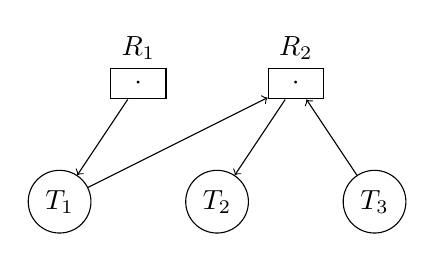
\begin{tikzpicture}
\tikzstyle{label} = [above,yshift=5pt];
\tikzstyle{res}=[minimum width=20pt,minimum height=5pt,draw];
\tikzstyle{pro}=[circle,draw];
\tikzstyle{alloc}=[->];
\node (v1) [res] at (-1,1) {$\cdot$};
\node [label] at (v1) {$R_1$};
\node [pro] (v2) at (-2,-0.5) {$T_1$};
\draw [alloc] (v1) edge (v2);

\node [pro] (v4) at (0,-0.5) {$T_2$};
\node [pro] (v5) at (2,-0.5) {$T_3$};
\node (v3) [res] at (1,1) {$\cdot$};
\node [label] at (v3) {$R_2$};
\draw [alloc] (v2) edge (v3);
\draw [alloc] (v3) edge (v4);
\draw [alloc] (v5) edge (v3);
\end{tikzpicture} & 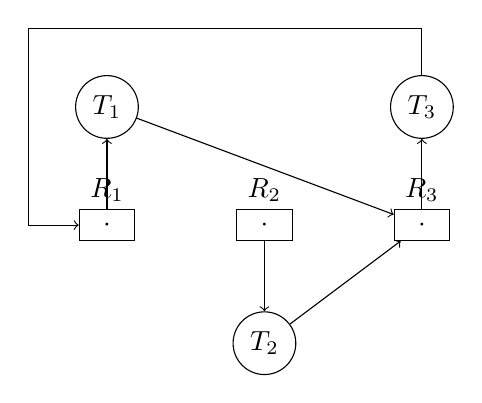
\begin{tikzpicture}
\tikzstyle{label} = [above,yshift=5pt];
\tikzstyle{res}=[minimum width=20pt,minimum height=5pt,draw];
\tikzstyle{pro}=[circle,draw];
\tikzstyle{alloc}=[->];
\node [res] (v1) at (-2,-2) {$\cdot$};
\node [label] at (v1) {$R_1$};
\node [pro] (v2) at (-2,-0.5) {$T_1$};
\draw [alloc] (v1) edge (v2);

\node [pro] (v4) at (0,-3.5) {$T_2$};
\node [pro] (v5) at (2,-0.5) {$T_3$};
\node [res] (v3) at (0,-2) {$\cdot$};
\node [label] at (v3) {$R_2$};
\node (v6) [res] at (2,-2) {$\cdot$};
\node [label] at (v6) {$R_3$};
\draw [alloc] (v6) edge (v5);
\draw [alloc] (v3) edge (v4);
\draw [alloc] (v2) edge (v6);
\draw [alloc] (v4) edge (v6);


\draw [alloc](v5) -- (2,0.5) -- (-3,0.5) -- (-3,-2) -- (v1);
\end{tikzpicture}\\
        \hline
        (c) & (d)\\
        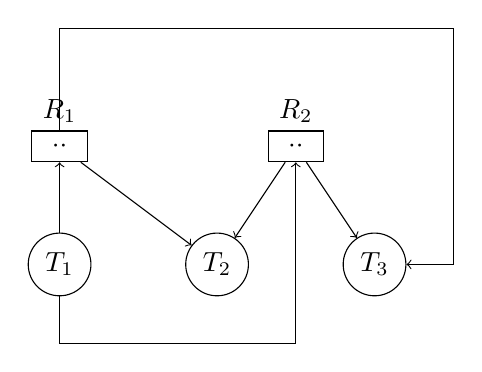
\begin{tikzpicture}
\tikzstyle{label} = [above,yshift=5pt];
\tikzstyle{res}=[minimum width=20pt,minimum height=5pt,draw];
\tikzstyle{pro}=[circle,draw];
\tikzstyle{alloc}=[->];
\node [res] (v1) at (-2,1) {$\cdot\cdot$};
\node [label] at (v1) {$R_1$};
\node [pro] (v2) at (-2,-0.5) {$T_1$};

\node [pro] (v4) at (0,-0.5) {$T_2$};
\node [pro] (v5) at (2,-0.5) {$T_3$};
\node [res] (v3) at (1,1) {$\cdot\cdot$};
\node [label] at (v3) {$R_2$};
\draw [alloc] (v2) edge (v1);
\draw [alloc] (v1) edge (v4);
\draw [alloc] (v3) edge (v4);
\draw [alloc] (v3) edge (v5);
\draw [alloc](v1) -- (-2,2.5) -- (3,2.5) -- (3,-0.5) -- (v5);
\draw [alloc](v2) -- (-2,-1.5) -- (1,-1.5) -- (v3);
\end{tikzpicture} & \input{img/d.tex}\\
        \hline
        (e) & (f)\\
        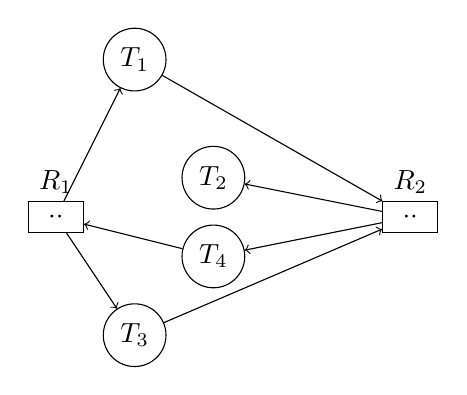
\begin{tikzpicture}
\tikzstyle{label} = [above,yshift=5pt];
\tikzstyle{res}=[minimum width=20pt,minimum height=5pt,draw];
\tikzstyle{pro}=[circle,draw];
\tikzstyle{alloc}=[->];
\node [res] (v1) at (-3,1) {$\cdot\cdot$};
\node [label] at (v1) {$R_1$};
\node [pro] (v2) at (-2,3) {$T_1$};

\node [pro] (v4) at (-1,1.5) {$T_2$};
\node [pro] (v5) at (-2,-0.5) {$T_3$};
\node [res] (v3) at (1.5,1) {$\cdot\cdot$};
\node [label] at (v3) {$R_2$};
\node [pro] (v6) at (-1,0.5) {$T_4$};
\draw [alloc] (v1) edge (v2);
\draw [alloc] (v2) edge (v3);
\draw [alloc] (v3) edge (v4);
\draw [alloc] (v5) edge (v3);
\draw [alloc] (v1) edge (v5);
\draw [alloc] (v3) edge (v6);
\draw [alloc] (v6) edge (v1);
\end{tikzpicture}
 & 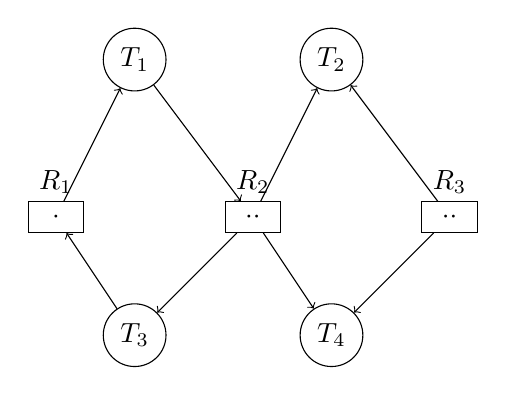
\begin{tikzpicture}
\tikzstyle{label} = [above,yshift=5pt];
\tikzstyle{res}=[minimum width=20pt,minimum height=5pt,draw];
\tikzstyle{pro}=[circle,draw];
\tikzstyle{alloc}=[->];
\node [res] (v1) at (-3,1) {$\cdot$};
\node [label] at (v1) {$R_1$};
\node [pro] (v2) at (-2,3) {$T_1$};

\node [pro] (v4) at (0.5,3) {$T_2$};
\node [pro] (v5) at (-2,-0.5) {$T_3$};
\node [res] (v3) at (-0.5,1) {$\cdot\cdot$};
\node [label] at (v3) {$R_2$};
\node [pro] (v6) at (0.5,-0.5) {$T_4$};
\draw [alloc] (v1) edge (v2);

\node (v7) [res] at (2,1) {$\cdot\cdot$};
\node [label] at (v7) {$R_3$};

\draw [alloc] (v2) edge (v3);
\draw [alloc] (v3) edge (v4);
\draw [alloc] (v7) edge (v4);
\draw [alloc] (v3) edge (v5);
\draw [alloc] (v5) edge (v1);
\draw [alloc] (v3) edge (v6);
\draw [alloc] (v7) edge (v6);
\end{tikzpicture}
\\
        \hline
    \end{tabular}

    \sol
        \begin{enumerate}[(a)]
            \item 等待图为
            
            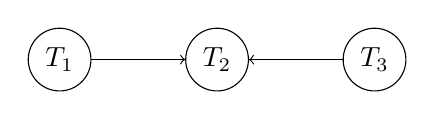
\begin{tikzpicture}
\tikzstyle{label} = [above,yshift=5pt];
\tikzstyle{res}=[minimum width=20pt,minimum height=5pt,draw];
\tikzstyle{pro}=[circle,draw];
\tikzstyle{alloc}=[->];
\node [pro] (v2) at (-2,-0.5) {$T_1$};

\node [pro] (v4) at (0,-0.5) {$T_2$};
\node [pro] (v5) at (2,-0.5) {$T_3$};
\draw [alloc] (v2) edge (v4);

\draw [alloc] (v5) edge (v4);
\end{tikzpicture}


            图中没有环,所以不会死锁。
            \item 等待图为
            
            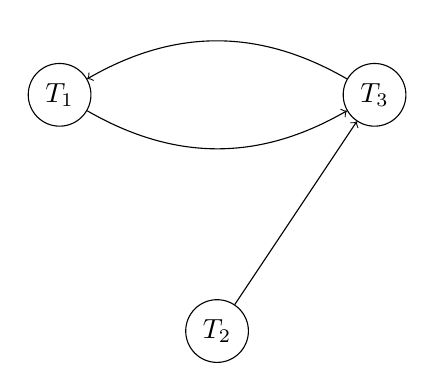
\begin{tikzpicture}
\tikzstyle{label} = [above,yshift=5pt];
\tikzstyle{res}=[minimum width=20pt,minimum height=5pt,draw];
\tikzstyle{pro}=[circle,draw];
\tikzstyle{alloc}=[->];
\node [pro] (v2) at (-2,-0.5) {$T_1$};

\node [pro] (v4) at (0,-3.5) {$T_2$};
\node [pro] (v5) at (2,-0.5) {$T_3$};


\draw [alloc,in=30,out=150] (v5) edge (v2);
\draw [alloc] (v4) edge (v5);
\draw [alloc,in=210,out=-30] (v2) edge (v5);
\end{tikzpicture}

            图中有环,所以会死锁。
            \item 虽然等待图中存在环$T_1\leftrightarrow T_2$,但是,如果将$T_2$释放,图中就不会存在死锁,所以该图不会死锁。
            \item 该图存在死锁,$T_1,T_2$ 请求 $R_2$ 而 $T_3,T_4$ 请求 $R_1$,资源已经都被占用。
            \item 该图不存在死锁,释放$T_2$,再释放$T_1$(或$T_3$)就不会导致死锁。
            \item $R_2$不足,左侧存在死锁,所以该图存在死锁。
        \end{enumerate}

    \item[8.27] Consider the following snapshot of a system:
     
    \begin{tabular}{cccc}
        & \underline{\emph{Allocation}} & \underline{\emph{Max}} & \underline{\textbf{\emph{Need}}}\\
        & $ABCD$ & $ABCD$ & $ABCD$ \\
   $T_0$ & 1202 & 4316 & 3114\\
   $T_1$ & 0112 & 2424 & 2312\\
   $T_2$ & 1240 & 3651 & 2411\\
   $T_3$ & 1201 & 2623 & 1422\\
   $T_4$ & 1001 & 3112 & 2111
   \end{tabular} 

   Using the banker's algorithm, determine whether or not each of the following states is unsafe. If the state is safe, illustrate the order in which the threads may complete. Otherwise, illustrate why the state is unsafe.
   \begin{steps}
    \item[a] \emph{Available}=(2,2,2,3)
     
    \sol \begin{tabular}{cc}
        Sequence  & \underline{\emph{Available}} \\
          & $A,B,C,D$ \\
      $T_4$ & 3,2,2,4 \\
      $T_0$ & 4,4,2,6 \\
      $T_3$ & 5,6,2,7 \\
      $T_1$ & 5,7,3,9 \\
      $T_2$ & 6,9,7,9
      \end{tabular} 

      存在安全序列 $\langle T_4,T_0,T_3,T_1,T_2 \rangle$,所以系统是安全的。
    \item[b] \emph{Available}=(4,4,1,1)
    
    \sol \begin{tabular}{cc}
        Sequence  & \underline{\emph{Available}} \\
          & $A,B,C,D$ \\
      $T_4$ & 5,4,1,2 \\
      $T_2$ & 6,6,5,2 \\
      $T_3$ & 7,8,5,3 \\
      $T_1$ & 7,9,6,5 \\
      $T_0$ & 8,11,6,7
      \end{tabular} 

      存在安全序列 $\langle T_4,T_2,T_3,T_1,T_0\rangle$,所以系统是安全的。
    \item[c] \emph{Available}=(3,0,1,4)
    
    \sol 都至少需要一个 $B$ 资源,所以处于不安全状态。

    \item[d] \emph{Available}=(1,5,2,2)   
    
    \sol  \begin{tabular}{cc}
        Sequence  & \underline{\emph{Available}} \\
          & $A,B,C,D$ \\
      $T_3$ & 2,7,2,3 \\
      $T_2$ & 3,9,6,3 \\
      $T_1$ & 3,10,7,5\\
      $T_0$ & 4,12,7,7\\
      $T_4$ & 5,12,7,8
      \end{tabular} 

      存在安全序列 $\langle T_3,T_2,T_1,T_0,T_4\rangle $,所以系统处于安全状态。
   \end{steps}
    \item[8.28] Consider the following snapshot of a system:
    
    \begin{tabular}{ccccc}
        & \underline{\emph{Allocation}} & \underline{\emph{Max}}  & \underline{\textbf{\emph{Need}}} &  \underline{\emph{Available}}\\
        & $ABCD$ & $ABCD$ & $ABCD$ & $ABCD$\\
   $T_0$ & 3141 & 6473& 3332 &2224\\
   $T_1$ & 2102 & 4232& 2130 &\\
   $T_2$ & 2413 & 2533& 0120 &\\
   $T_3$ & 4110 & 6332& 2222 &\\
   $T_4$ & 2221 & 5675& 3454 &
   \end{tabular} 

   Answer the following questions using the banker's algorithm:
   \begin{steps}
       \item[a] Illustrate that the system is in a safe state by demonstrating an order in which the threads may complete.
       
       \sol \begin{tabular}{cc}
        Sequence  & \underline{\emph{Available}} \\
          & $A,B,C,D$ \\
      $T_2$ & 4,6,3,7 \\
      $T_3$ & 8,7,4,7 \\
      $T_1$ & 10,8,4,8 \\
      $T_0$ & 13,9,8,9 \\
      $T_4$ & 16,13,13,13
      \end{tabular} 

      安全序列为 $\langle T_2,T_3,T_1,T_0,T_4 \rangle$。
       \item[b] If a request from thread $T_4$ arrives for (2,2,2,4), can the request begranted immediately?
       
       \ans 不可以,会导致资源耗尽,但没有释放,所有的进程都不能进行完毕。
       \item[c] If a request from thread $T_2$ arrives for (0,1,1,0), can the request begranted immediately?
       
       \ans 可以,只要继续完成 $T_2$,就可以按照相同的安全序列完成所有任务。
       \item[d] If a request from thread $T_3$ arrives for (2,2,1,2), can the request begranted immediately?
       
       \ans 可以,只要继续完成 $T_3$,就可以按照安全序列 $\langle T_3,T_2,T_1,T_0,T_4 \rangle$完成任务。
   \end{steps}
\end{problems}

\end{document}